 \section{Unidad 1}

\subsection{L1. El espacio geográfico}

\ejemplosboxed[4]{Relaciona cada saber ancestral con el recurso que aprovecha y conserva al mismo tiempo.

\vspace{0.5cm}
\begin{minipage}[c]{0.6\textwidth}
\begin{parts}
        \part Cría de abejas meliponas: \dashfill \fillin[3][0.5cm]

    \part Medicina tradicional: \dashfill \fillin[4][0.5cm]

\part Agricultura de temporal: \dashfill \fillin[1][0.5cm]

    \part Construcción de chinampas: \dashfill \fillin[2][0.5cm]

\end{parts}
\end{minipage} 
\hfill
\begin{minipage}[c]{0.35\textwidth}
    \begin{enumerate}
    \item Conocimiento del clima 
    \item Canales lacustres 
    \item Fauna nativa 
    \item Plantas medicinales
    \end{enumerate}
\end{minipage}
}


\questionboxed[4]{Elige si los siguientes saberes o técnicas son de origen \textbf{Ancestral} o \textbf{Moderno}.

% \begin{multicols}{2}
\begin{parts}
    \part Relación de cultivos en la milpa. \fillin[Ancestral][2cm]

    \part Hidroponia. \fillin[Moderno][2cm]

    \part Uso de sistemas de riego por bombeo. \fillin[Moderno][2cm]

    \part Consumo de alimentos locales y de temporada. \fillin[Ancestral][2cm]
\end{parts}
% \end{multicols}
}

\subsection{L2. Categorías de análisis del espacio geográfico}

\ejemplosboxed[8]{Elige la categoría de análisis del espacio geográfico que utilizarías para realizar los siguientes estudios.

\vspace{0.5cm}
\begin{minipage}[c]{0.8\textwidth}
\begin{parts}
    \part Jardín Escultórico de Edward James en Xilitla. \dashfill \fillin[2][0.5cm]
    
    \part Campos de viñedos a los pies de la Cordillera de los Andes en Chile. \dashfill \fillin[1][0.5cm]
    
    \part Aprovechamiento de los recursos naturales para el turismo en Jalcomulco. \dashfill \fillin[2][0.5cm]
    
    \part Contaminación de las playas en la Costa Grande de Guerrero. \dashfill \fillin[3][0.5cm]
    
    \part Municipios y disponibilidad de agua en Sonora. \dashfill \fillin[4][0.5cm]
    
    \part Predominio industrial en Naucalpan, Estado de México. \dashfill \fillin[1][0.5cm]
    
    \part Países que hablan alguna lengua de origen latino en América. \dashfill \fillin[3][0.5cm]
    
    \part Organización política de algunos países en Europa. \dashfill \fillin[4][0.5cm]
    
\end{parts}
\end{minipage} 
\hfill
\begin{minipage}[c]{0.15\textwidth}
    \begin{enumerate}
    \item Paisaje \\
    \item Lugar \\
    \item Región \\
    \item Territorio 
    \end{enumerate}
\end{minipage}
}


\questionboxed[8]{Elige la palabra correcta del menú que complete los siguientes enunciados:

\begin{center}
\wordpill{lugar}
\wordpill{territorio}
\wordpill{paisaje}
\wordpill{región}
\end{center}

\begin{parts}
    \part Cayman Lodge Amazonia es un \fillin[lugar][2cm] en la Amazonia. Se localiza en el \fillin[territorio][2cm] de Perú.

    \part En las fotografías del \fillin[paisaje][2cm] de la selva amazónica, uno de los elementos principales es el río.

    \part La Amazonia abarca parte del \fillin[territorio][2cm] de Brasil, Bolivia y Colombia, entre otros países.

    \part Parte del proyecto de Cayman Lodge Amazonia es la protección de esta \fillin[región][2cm], que es considerada ``el pulmón principal'' de nuestro planeta.

    \part En el \fillin[paisaje][2cm] selvático de esta \fillin[región][2cm] natural predomina el componente natural de espacio geográfico.

    \part En este \fillin[lugar][2cm] llamado Cayman Lodge se puede convivir directamente con la naturaleza.

\end{parts}
}




\subsection{L3. El estudio del espacio geográfico }

\ejemplosboxed[4]{Relaciona las definiciones con el elemento que le corresponde.

\begin{minipage}[t]{0.25\textwidth}
    \begin{enumerate}
        \item \wordpill{Dron}
        \item \wordpill{Imágenes de satélite}
        \item \wordpill{Mapas digitales}
        \item \wordpill{GPS}
    \end{enumerate}
\end{minipage}
\hfill
\begin{minipage}[t]{0.7\textwidth}
    \begin{parts}
        \part (\fillin[3][0.25cm]) A través de la tecnología informática es posible almacenar, procesar y analizar información para la representación espacial.
        \part (\fillin[2][0.25cm]) Su aplicación es frecuente en el estudio de las condiciones atmosféricas de una región.
        \part (\fillin[4][0.25cm]) Permite posicionar con precisión lugares, objetos, personas y vehículos sobre la superficie terrestre.
        \part (\fillin[1][0.25cm]) Dispositivo móvil auxiliar para estudiar los componentes de espacios geográficos de difícil acceso.
    \end{parts}
\end{minipage}

}

\questionboxed[5]{Elige la característica del espacio geográfico que le corresponde a cada descripción.

\begin{center}
\wordpill{Distribución}
\wordpill{Cambio}
\wordpill{Relación}
\wordpill{Localización}
\wordpill{Diversidad}
\end{center}

\begin{parts}
    \part \fillin[Localización][2cm] Las coordenadas de Los Ángeles, California, en Estados Unidos de América, son: 34° 03' Norte; 118° 15' Oeste. 
    \part \fillin[Cambio][2cm] Santa Fe es una colonia de la Ciudad de México que hasta los años treinta era una zona de minas de arena, y en la actualidad es uno de los centros financieros más importantes del país. 
    \part \fillin[Diversidad][2cm] Las selvas, desiertos, bosques y mares forman parte de los ecosistemas que podemos encontrar en México. 
    \part \fillin[Relación][2cm] En la Vega de Metztitlán, Hidalgo, la riqueza del suelo es favorecida por las crecientes del Río Venados, lo que permite una gran producción agrícola. 
    \part \fillin[Distribución][2cm] En los estados del norte del país se concentra el mayor número de maquiladoras. Dichos estados son: Baja California, Chihuahua, Tamaulipas, Coahuila de Zaragoza, Sonora y Nuevo León. 
\end{parts}
}

\subsection{L4. Representaciones cartográficas }

\ejemplosboxed[6]{Observa la fotografía aérea agrícola y elige la respuesta correcta:

\begin{center}
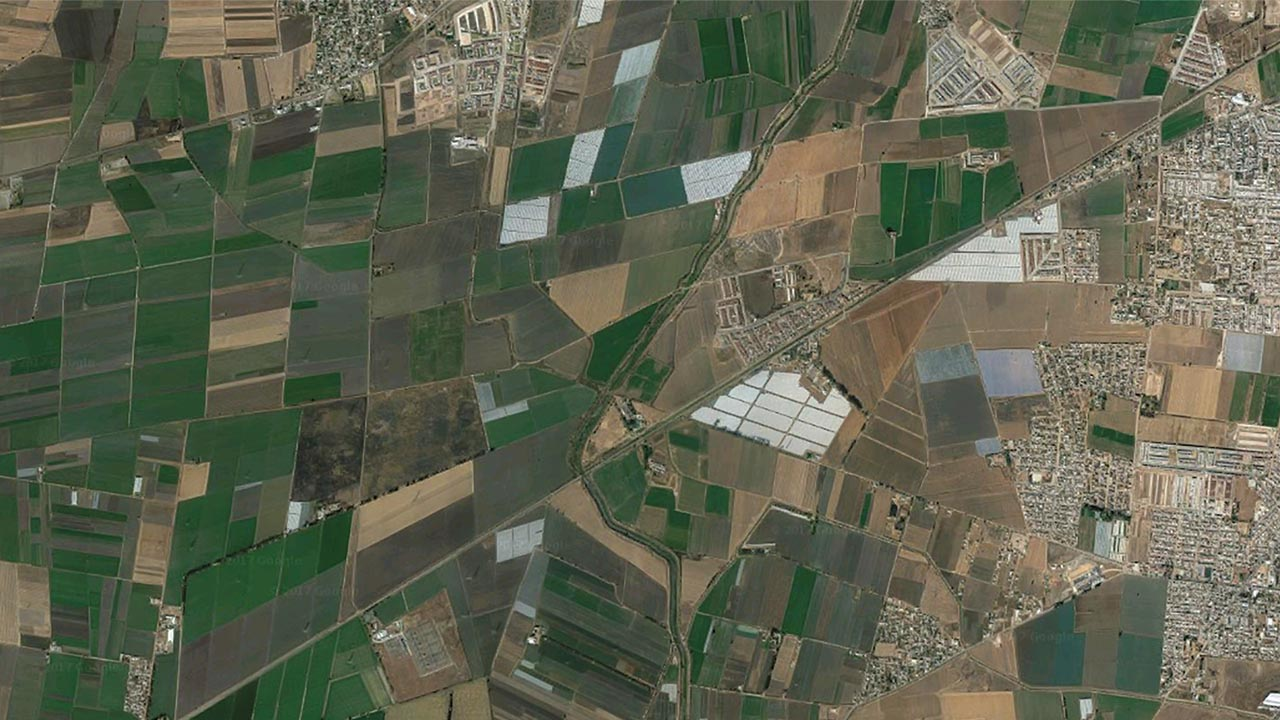
\includegraphics[width=0.7\linewidth]{../images/SIMGE-SB-L1-U1-LEC4-04-IMG-01.jpg}
\end{center}
               
\begin{parts}
    \part ¿Qué representan los recuadros verdes en la fotografía aérea?
    
    \begin{oneparchoices}
        \choice Las localidades \CorrectChoice Los cultivos \choice La vegetación \choice Los cuerpos de agua
    \end{oneparchoices}
  
    \part ¿Qué representan los recuadros blancos?
  
    \begin{oneparchoices}
        \choice Las carpas \choice Las fábricas \choice Las casas \CorrectChoice Los invernaderos
    \end{oneparchoices}
   
    \part ¿Qué representan las líneas rectas?
   
    \begin{oneparchoices}
        \choice Los canales de riego \choice Las vías del tren \choice Los ríos \CorrectChoice Las carreteras
    \end{oneparchoices}
\end{parts}
}


\questionboxed[6]{Coloca las palabras para completar las afirmaciones sobre fotografías aéreas.


 \begin{center}
        \wordpill{calles} 
            \wordpill{drones}  
\wordpill{aviación}
           \wordpill{satélite}
     \wordpill{reconocer}    
       \wordpill{componentes} 
    \end{center}

\begin{parts}
    \part La \fillin[aviación][2cm] y la fotografía son inventos que permiten la toma de fotografías aéreas.
    
    \part En la actualidad, con las fotografías aéreas se pueden \fillin[reconocer][2.5cm] las zonas urbanas, los poblados, la vegetación, el trazo de las \fillin[calles][2cm] y todos los \fillin[componentes][2.5cm] del espacio geográfico.
  
    \part En la actualidad las fotografías aéreas están siendo sustituidas por fotografías tomadas con \fillin[drones][2cm] o por imágenes tomadas desde un \fillin[satélite][2.5cm].
\end{parts}
}


\questionboxed[6]{Elige la categoría que corresponde a la característica o ejemplo de los tipos de símbolos.

\vspace{0.5cm}
\begin{minipage}[c]{0.6\textwidth}
\begin{parts}
     \part En esta categoría entran las superautopistas y se utilizan diferentes colores para indicar su importancia. \dashfill  \fillin[2][0.5cm]

    \part En los mapas topográficos se utilizan para la representación de ciudades. \dashfill \fillin[3][0.5cm]

    \part Son ideales para la representación de regiones naturales, tipos de climas o cuerpos de agua como los océanos. \dashfill \fillin[3][0.5cm]

    \part Representan elementos aislados del espacio geográfico de importancia para la orientación de los lugares. \dashfill \fillin[1][0.5cm]

    \part Representan límites de tipo natural o social, como las fronteras entre los países. \dashfill  \fillin[2][0.5cm]

    \part Los hospitales utilizan este tipo de símbolos para su ubicación exacta en el mapa y poder ser ubicados rápidamente. \dashfill \fillin[1][0.5cm]
    
\end{parts}
\end{minipage} 
\hfill
\begin{minipage}[c]{0.25\textwidth}
    \begin{enumerate}
    \item Puntuales \\
    \item Lineales \\
    \item De área 
    \end{enumerate}
\end{minipage}
}

\questionboxed[7]{Relaciona el significado de los glifos representados en el mapa histórico de Mixquiahuala con el número que corresponda según la figura.

\begin{minipage}[c]{0.75\textwidth}

               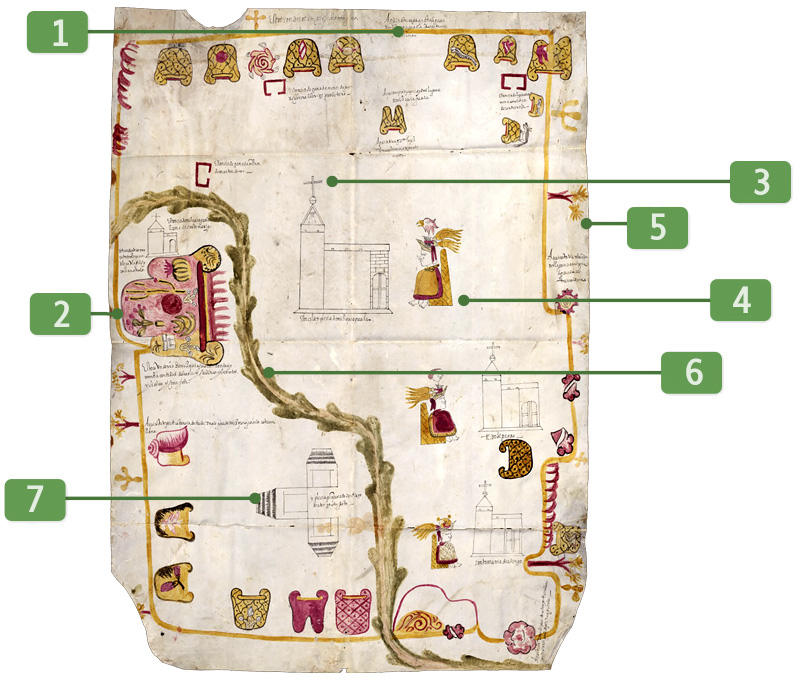
\includegraphics[width=\linewidth]{../images/espacio_geografico_01.png}
\end{minipage} 
\hfill
\begin{minipage}[c]{0.2\textwidth}
\begin{parts}
      \part \fillin[5][0.5cm] Vegetación \\

    \part \fillin[3][0.5cm] Iglesia \\

        \part \fillin[6][0.5cm] Río \\

        \part \fillin[7][0.5cm] Casas \\

    \part \fillin[2][0.5cm] Montaña \\

  \part \fillin[1][0.5cm] Línea de límite \\

        \part \fillin[4][0.5cm] Gobernante \\
\end{parts}
\end{minipage} 

}





\subsection{L5. Interpretación y representación de la Información geográfica}

\ejemplosboxed[5]{De acuerdo con el mapa de Atracción y expulsión de migrantes, responde lo siguiente:

\begin{multicols}{2}

\begin{parts}
    
 
    \part Es uno de los principales destinos de los emigrantes de China.
  
    \begin{oneparchoices}
        \choice Francia \choice México \CorrectChoice Canadá \choice Reino Unido
    \end{oneparchoices}
  
    
 
    \part ¿En qué continente predominan los países con desplazamientos internos de migrantes?
  
    \begin{oneparchoices}
        \choice América \choice Europa \choice Asia \CorrectChoice África
    \end{oneparchoices}

\part China presenta una expulsión de migrantes de tipo:
  
    \begin{oneparchoices}
        \CorrectChoice Fuerte \choice Medio \choice Débil \choice Escasa
    \end{oneparchoices}

\part ¿Cuál es el principal destino de los brasileños?
  
    \begin{oneparchoices}
        \choice Australia \CorrectChoice Japón \choice Inglaterra \choice México
    \end{oneparchoices}

\part ¿Qué nivel de atracción tienen los países de América del Norte?
   
    \begin{oneparchoices}
        \CorrectChoice Fuerte \choice Medio \choice Débil \choice Escasa
    \end{oneparchoices}
\end{parts}
\end{multicols}
}

\questionboxed[3]{Señala si son \textit{verdaderas} o \textit{falsas} las afirmaciones sobre los usos o aplicaciones de los mapas.

\begin{multicols}{2}
\begin{parts}
    \part Se utilizan para el trazado de rutas y localización de lugares de desastre.

\begin{oneparchoices}
                         \CorrectChoice Verdadero \choice Falso
                    \end{oneparchoices}
                    
    \part  Los utilizan los gobiernos para delimitar predios y cobrar por el uso de suelo.

\begin{oneparchoices}
                         \CorrectChoice Verdadero \choice Falso
                    \end{oneparchoices}
                    
    \part  Determinan rutas de evacuación en caso de una erupción volcánica.

\begin{oneparchoices}
                         \CorrectChoice Verdadero \choice Falso
                    \end{oneparchoices}
               
                    \columnbreak%

    \part  Representan información en tiempo real de un desastre ocasionado por un sismo.

\begin{oneparchoices}
                         \choice Verdadero \CorrectChoice Falso
                    \end{oneparchoices}
                 
                     \part  Con ellos se pueden ubicar de manera precisa y exacta las coordenadas de un punto sobre la superficie terrestre.

\begin{oneparchoices}
                         \choice Verdadero \CorrectChoice Falso
                    \end{oneparchoices}

    \part  Gracias a ellos, se pueden determinar alturas aproximadas de elementos del relieve.

\begin{oneparchoices}
                         \CorrectChoice Verdadero \choice Falso
                    \end{oneparchoices}

\end{parts}
\end{multicols}
}




\subsection{L6. Tecnologías de la información geográfica}

\ejemplosboxed[9]{Completa el siguiente párrafo sobre las tecnologías utilizadas en el manejo de información geográfica con las palabras correspondientes:

    \begin{center}
        \wordpill{espacio}  
        \wordpill{satelital} 
        \wordpill{personas} 
        \wordpill{GPS}
        \wordpill{software}
        \wordpill{SIG} 
        \wordpill{drones}
        \wordpill{información}
        \wordpill{tecnologías}    
    \end{center}

En la actualidad existen diversas técnicas, métodos y \fillin[tecnologías][2cm] para obtener y procesar \fillin[información][2cm]  del \fillin[espacio][2cm] geográfico. Dentro del tipo de tecnologías utilizadas para este fin se encuentran los equipos  \fillin[GPS][2cm], los \fillin[SIG][2cm], las imágenes de satélite y los vehículos aéreos tripulados de manera remota, también llamados \fillin[drones][1cm]. El GPS se utiliza para conocer la ubicación de los lugares, los objetos o las \fillin[personas][2cm]; por su parte, los SIG se componen de una computadora y un \fillin[software][2cm] o programa especializado útil para el análisis y procesamiento de la información obtenida de forma \fillin[satelital][2cm] o aérea.
}

\questionboxed[6]{Clasifica las siguientes características indicando si pertenecen a un Sistema de Posicionamiento Global (\textbf{GPS}) o a un Sistema de Información Geográfica (\textbf{SIG}).

\begin{parts}
    \part \fillin[GPS][1cm] Permite posicionar con gran precisión puntos sobre la superficie de la Tierra.
    \part \fillin[SIG][1cm] Por medio de esta herramienta se puede utilizar la información registrada en bases de datos geográficos.
    \part \fillin[GPS][1cm] Sus siglas en inglés equivalen a Sistema de Posicionamiento Global.
    \part \fillin[SIG][1cm] Sus siglas significan Sistema de Información Geográfica.
    \part \fillin[GPS][1cm] Al inicio fue desarrollado con fines militares por Estados Unidos de América.
    \part \fillin[SIG][1cm] Son sistemas computarizados por medio de los cuales se pueden realizar mapas de diversos temas.
\end{parts}
}


\questionboxed[4]{Elige el sistema (GPS o SIG) que permite llevar a cabo las siguientes aplicaciones:

\begin{parts}
    \part \fillin[SIG][1cm] Monitorear especies animales en peligro de extinción.
    \part \fillin[GPS][1cm] Trasladarse de un lugar a otro en la vida cotidiana.
    \part \fillin[SIG][1cm] Considerar diferentes elementos para establecer un Área Natural Protegida.
    \part \fillin[SIG][1cm] Planear espacios urbanos con el objetivo de tener una mejor organización y funcionalidad.
    \part \fillin[SIG][1cm] Crear escenarios inexistentes para simular algún suceso, como una erupción volcánica o un huracán.
    \part \fillin[GPS][1cm] Trazar rutas de navegación terrestres, marítimas y aéreas.
    \part \fillin[GPS][1cm] Proporcionar datos correspondientes a la latitud, longitud y altitud (coordenadas).
\end{parts}
}

\questionboxed[4]{Elige si las funciones de un SIG descritas son Verdaderas (V) o Falsas (F).

\begin{multicols}{2}
\begin{parts}
    \part En Europa se dio a conocer el primer Sistema de Información Geográfica (SIG).
    
    \begin{oneparchoices}
                         \choice Verdadero \CorrectChoice Falso
                    \end{oneparchoices}

    \part Los SIG integran un conjunto de herramientas para almacenar y analizar información acerca de las características del espacio geográfico.
   
    \begin{oneparchoices}
                         \CorrectChoice Verdadero \choice Falso
                    \end{oneparchoices}

    \part  Un mapa representa la realidad en la que vivimos.
    
    \begin{oneparchoices}
                         \choice Verdadero \CorrectChoice Falso
                    \end{oneparchoices}

    \part Un SIG contiene toda la información geográfica de todo el mundo.
    
       \begin{oneparchoices}
                         \choice Verdadero \CorrectChoice Falso
                    \end{oneparchoices}

    \part Los SIG tienen un funcionamiento que opera mediante diferentes módulos.
    
    \begin{oneparchoices}
                         \CorrectChoice Verdadero \choice Falso
                    \end{oneparchoices}

    \part Los módulos de los SIG son de entrada, almacenamiento, salida y manejo de información.
    
    \begin{oneparchoices}
                         \CorrectChoice Verdadero \choice Falso
                    \end{oneparchoices}

    \part La función de los SIG es la misma y se puede ver de igual forma en diferentes partes del mundo.
    
      \begin{oneparchoices}
                         \choice Verdadero \CorrectChoice Falso
                    \end{oneparchoices}

    \part  Los SIG guardan su información en una base de datos geográficos dentro de un sistema.
    
    \begin{oneparchoices}
                         \CorrectChoice Verdadero \choice Falso
                    \end{oneparchoices}

\end{parts}
\end{multicols}

}




\ejemplosboxed[7]{Ordena los procesos utilizados por un GPS para el trazado de una ruta.

\begin{parts}
      \part \fillin[3][1cm] Señalar el lugar donde deseas ir.
   \part \fillin[1][1cm] Tener un aparato receptor de señal GPS, por ejemplo, un celular.      
  \part \fillin[5][1cm] Por medio de un algoritmo, el software calcula distancias y tiempos de recorrido.
   \part \fillin[6][1cm] El software señala la ruta a seguir en imagen.
 \part \fillin[2][1cm] Ubicar el lugar donde te encuentras.
  \part \fillin[4][1cm] El celular por medio de un software especializado procesa la información.    
  \part \fillin[7][1cm] El usuario se puede trasladar al lugar deseado.
\end{parts}
}

\questionboxed[7]{Ordena los procesos utilizados por un GPS para el trazado de una ruta.

\begin{parts}
        \part \fillin[4][1cm] El celular por medio de un software especializado procesa la información.
   \part \fillin[6][1cm] El software señala la ruta a seguir en imagen.
  \part \fillin[3][1cm] Señalar el lugar donde deseas ir.
      \part \fillin[7][1cm] El usuario se puede trasladar al lugar deseado.
       \part \fillin[1][1cm] Tener un aparato receptor de señal GPS, por ejemplo, un celular.
 \part \fillin[5][1cm] Por medio de un algoritmo, el software calcula distancias y tiempos de recorrido.
 \part \fillin[2][1cm] Ubicar el lugar donde te encuentras.
\end{parts}
}
\subsection{L7. Las placas tectónicas y su relación con la sismicidad y el vulcanismo}

\ejemplosboxed[5]{Completa los siguientes enunciados con la forma de relieve o concepto correspondiente:

 \begin{center}
        \wordpill{del relieve}  
        \wordpill{montañas} 
        \wordpill{mesetas} 
        \wordpill{llanuras}
        \wordpill{depresiones}  
    \end{center}

\begin{parts}
    \part En las formas generales \fillin[del relieve][2.5cm] intervienen procesos internos y externos de la Tierra; unos intervienen en su formación y otros en su modelación.
    \part Las \fillin[montañas][2.5cm] pueden alcanzar alturas entre los 1 000 a 8 000 metros sobre el nivel medio del mar en promedio.
    \part Las \fillin[mesetas][2.5cm] o altiplanicies son áreas llanas o de terreno con poca pendiente situadas a cierta altitud.
    \part Las \fillin[llanuras][2.5cm] o planicies son zonas extensas de poca altitud.
    \part Las \fillin[depresiones][2.5cm] son partes del terreno hundidas que regularmente están ocupadas por agua.
\end{parts}
}

\questionboxed[5]{Indica si son Verdaderas (V) o Falsas (F) las afirmaciones con relación a la distribución de las regiones volcánicas.

\begin{multicols}{2}

\begin{parts}
    \part El centro de México, específicamente la región fisiográfica del Sistema Volcánico Transversal, es una de las más activas del mundo.

     \begin{oneparchoices}
                         \choice Verdadero \CorrectChoice Falso
                    \end{oneparchoices}
    \part Uno de los beneficios del vulcanismo son las aguas termales como atractivo turístico.

     \begin{oneparchoices}
                         \CorrectChoice Verdadero \choice Falso
                    \end{oneparchoices}
    \part En la región del Atlántico se localiza una dorsal oceánica que atraviesa la Tierra de sur a norte y es donde se localizan los volcanes de Islandia.

     \begin{oneparchoices}
                         \CorrectChoice Verdadero \choice Falso
                    \end{oneparchoices}
    \part A partir del vulcanismo se puede generar energía termoeléctrica.

     \begin{oneparchoices}
                         \choice Verdadero \CorrectChoice Falso
                    \end{oneparchoices}
    \part México y Japón son países que aprovechan el vulcanismo para la generación de energía eléctrica.

     \begin{oneparchoices}
                         \CorrectChoice Verdadero \choice Falso
                    \end{oneparchoices}
\end{parts}

\end{multicols}
}






\subsection{L8. Las placas tectónicas y su relación con el relieve}

\ejemplosboxed[10]{Elige la clase de erosión a la que se refieren las descripciones.

\begin{multicols}{2}
\begin{parts}
    \part Los profundos valles en forma de "V", originados por el paso constante de corrientes de agua dulce desde las montañas, son producto de la erosión...     
    
        \begin{oneparchoices}
        \choice Eólico
        \CorrectChoice Fluvial
        \choice Marítimo
        \end{oneparchoices}

    \part Ocurre en vastos desiertos como el Sahara, donde las partículas de arena son transportadas grandes distancias. 
    
    \begin{oneparchoices}
    \CorrectChoice Eólico
    \choice Fluvial
    \choice Marítimo
    \end{oneparchoices}

        \part Por esta clase de erosión se esculpió el famoso Gran Cañón del Colorado a lo largo de millones de años.  
    
        \begin{oneparchoices}
        \choice Eólico
        \CorrectChoice Fluvial
        \choice Marítimo
        \end{oneparchoices}

  \part El arrastre de la capa fértil del suelo agrícola debido al escurrimiento superficial del agua después de fuertes tormentas es un efecto de la erosión...
       
        \begin{oneparchoices}
        \choice Eólico
        \CorrectChoice Fluvial
        \choice Marítimo
        \end{oneparchoices} 

        \part Es el proceso responsable de esculpir las "rocas hongo" al golpear las bases de las formaciones rocosas con partículas en suspensión. 
    
        \begin{oneparchoices}
        \CorrectChoice Eólico
        \choice Fluvial
        \choice Marítimo
        \end{oneparchoices}

         \part Tiene la capacidad de formar cavernas costeras y arcos de roca debido al constante embate de las olas.  
    
        \begin{oneparchoices}
        \choice Eólico
        \choice Fluvial
        \CorrectChoice Marítimo
        \end{oneparchoices}

        \part El impacto constante de la precipitación sobre superficies sin vegetación reblandece la tierra, lo que provoca el desgaste del suelo. 
    
        \begin{oneparchoices}
        \choice Eólico
        \CorrectChoice Fluvial
        \choice Marítimo
        \end{oneparchoices}

        \part La formación del famoso "Arco" en Cabo San Lucas es resultado combinado del escurrimiento continental y el choque de las mareas, producto de la erosión...  
        
        \begin{oneparchoices}
        \choice Eólico
        \CorrectChoice Fluvial
        \CorrectChoice Marítimo
        \end{oneparchoices}

    
        \part El proceso de deflación, mediante el cual las corrientes de aire barren las partículas sueltas en planicies y laderas áridas, pertenece a este tipo de erosión. 
    
        \begin{oneparchoices}
        \CorrectChoice Eólico
        \choice Fluvial
        \choice Marítimo
        \end{oneparchoices}

      
        \part Dicha clase de erosión es la responsable de depositar sedimentos para la formación de deltas en la desembocadura de las corrientes de agua.     
    
        \begin{oneparchoices}
        \choice Eólico
        \CorrectChoice Fluvial
        \choice Marítimo
        \end{oneparchoices}

    \end{parts}
\end{multicols}
}

\questionboxed[5]{Elige la clase de erosión a la que se refieren las descripciones.

\begin{multicols}{2}
\begin{parts}
     \part Los fiordos, como los de Noruega, también son causa de la erosión...     
    
        \begin{oneparchoices}
        \choice Eólico
        \CorrectChoice Fluvial
        \choice Marítimo
        \end{oneparchoices}

    \part Ocurre principalmente en las regiones desérticas, como en el norte de México. 
    
    \begin{oneparchoices}
    \CorrectChoice Eólico
    \choice Fluvial
    \choice Marítimo
    \end{oneparchoices}

        \part Por esta clase de erosión se modeló el Cañón del Sumidero en Chiapas.  
    
        \begin{oneparchoices}
        \choice Eólico
        \CorrectChoice Fluvial
        \choice Marítimo
        \end{oneparchoices}

  \part Cuando se presenta una lluvia torrencial y el agua acarrea el material en corrientes similares a ríos, se habla de una erosión...
       
        \begin{oneparchoices}
        \choice Eólico
        \CorrectChoice Fluvial
        \choice Marítimo
        \end{oneparchoices} 

        \part Es la principal causa de que se formen las dunas y se modifiquen constantemente. 
    
        \begin{oneparchoices}
        \CorrectChoice Eólico
        \choice Fluvial
        \choice Marítimo
        \end{oneparchoices}

         \part Tiene la capacidad de formar acantilados.  
    
        \begin{oneparchoices}
        \choice Eólico
        \choice Fluvial
        \CorrectChoice Marítimo
        \end{oneparchoices}

        \part Las gotas de agua caen con gran velocidad y fuerza, lo que provoca el desgaste del suelo. 
    
        \begin{oneparchoices}
        \choice Eólico
        \CorrectChoice Fluvial
        \choice Marítimo
        \end{oneparchoices}

        \part Por causa de este tipo de erosión se ha formado el relieve característico de los Cabos en la Península de Baja California, en México.  
        
        \begin{oneparchoices}
        \choice Eólico
        \CorrectChoice Fluvial
        \CorrectChoice Marítimo
        \end{oneparchoices}

    
        \part En las montañas, principalmente, no existe vegetación y sus laderas se ven modeladas por este tipo de erosión. 
    
        \begin{oneparchoices}
        \CorrectChoice Eólico
        \choice Fluvial
        \choice Marítimo
        \end{oneparchoices}

      
        \part Dicha clase de erosión también puede formar meandros en los ríos.     
    
        \begin{oneparchoices}
        \choice Eólico
        \CorrectChoice Fluvial
        \choice Marítimo
        \end{oneparchoices}

    \end{parts}
\end{multicols}
}

\subsection{L9. El suelo y su importancia}


\ejemplosboxed[5]{Relaciona con una línea la descripción con el concepto que le corresponde.

\vspace{0.5cm}
\begin{minipage}[c]{0.4\textwidth}
% \begin{multicols}{2}
\begin{parts}
        \part Erosión hídrica  \dashfill \fillin[4][0.5cm] \\[-0.45em]

        \part Erosión eólica  \dashfill \fillin[3][0.5cm] \\[-0.45em]

        \part Erosión antrópica  \dashfill \fillin[5][0.5cm] \\[-0.45em]

        \part Suelo  \dashfill \fillin[1][0.5cm] \\[-0.45em]

        \part Consecuencias de la erosión del suelo \dashfill  \fillin[2][0.5cm] \\[-0.45em]

    \end{parts}
\end{minipage} 
\hfill
\begin{minipage}[c]{0.6\textwidth}
    \begin{enumerate}
    \item Es la capa superior de la superficie terrestre.
    \item Es la reducción de la productividad de los cultivos y afectación negativa a los agricultores.
    \item Es causada por el viento en zonas desérticas, la cual forma dunas.
    \item Es causada por los ríos, la cual forma cañones.
    \item Es generada por las actividades humanas como la minería.
    \end{enumerate}
\end{minipage}
% \end{multicols}
}

\questionboxed[3]{Completa los enunciados sobre el suelo:

 \begin{center}
       \wordpill{externos} 
       \wordpill{físicos}    
        \wordpill{ecosistémicos}  
         \wordpill{biológicos} 
        \wordpill{mezcla}
         \wordpill{lento}
    \end{center}

\begin{parts}
    \part El suelo se forma debido a los procesos \fillin[externos][2cm] de la Tierra.

    \part Los suelos aportan servicios \fillin[ecosistémicos][3cm] que permiten la vida en la Tierra.

    \part El suelo es una \fillin[mezcla][2cm] de minerales, materia orgánica, agua, seres vivos y aire.

    \part El proceso de formación del suelo es muy \fillin[lento][2cm] y depende de varios factores químicos, \fillin[biológicos][2.5cm] y \fillin[físicos][2.5cm].

\end{parts}
}


 \ejemplosboxed[6]{Señala si son \textit{verdaderas} o \textit{falsas} las siguientes frases:
         
          \begin{multicols}{2}
               \begin{parts}
                    \part La degradación del suelo reduce la calidad y cantidad de hábitats disponibles para las especies, lo que puede llevar a una disminución de la biodiversidad.

                    \begin{oneparchoices}
                         \CorrectChoice Verdadero \choice Falso
                    \end{oneparchoices}

                    \part La pérdida de suelo fértil aumenta la cantidad de alimento disponible para los animales y plantas, lo que puede mejorar su supervivencia y reproducción.

                    \begin{oneparchoices}
                         \choice Verdadero \CorrectChoice Falso
                    \end{oneparchoices}

                    \columnbreak%

     \part La pérdida del suelo sólo se presenta en las regiones desérticas de México, principalmente la de tipo eólica.

                    \begin{oneparchoices}
                         \choice Verdadero \CorrectChoice Falso
                    \end{oneparchoices}

                    \part La erosión del suelo y la degradación de la tierra alteran el hábitat de los seres vivos que viven en el suelo, como las lombrices de tierra, los insectos y los microorganismos.

                    \begin{oneparchoices}
                         \CorrectChoice Verdadero \choice Falso
                    \end{oneparchoices}
               \end{parts}
          \end{multicols}
     }

\questionboxed[4]{Señala si son \textit{verdaderas} o \textit{falsas} las afirmaciones sobre el daño o beneficio del suelo.

\begin{multicols}{2}
\begin{parts}
    \part La composta desfavorece la fertilización del suelo.

     \begin{oneparchoices}
                         \choice Verdadero \CorrectChoice Falso
                    \end{oneparchoices} 
                    
                    \part El uso de agroquímicos en la agricultura beneficia los suelos.

     \begin{oneparchoices}
                         \choice Verdadero \CorrectChoice Falso
                    \end{oneparchoices}

                    \columnbreak%

    \part El problema más común que afecta al suelo es la erosión.

     \begin{oneparchoices}
                         \CorrectChoice Verdadero \choice Falso
                    \end{oneparchoices}


    \part La deforestación tiene un impacto negativo sobre el suelo.

     \begin{oneparchoices}
                         \CorrectChoice Verdadero \choice Falso
                    \end{oneparchoices}
\end{parts}
\end{multicols}
}



\subsection{L10. Aguas continentales en México y el mundo }

\ejemplosboxed[9]{

\begin{parts}
\part Anota una \checkmark en las afirmaciones con las que estés de acuerdo. Guíate con lo que aprendiste en esta lección y en tu libro de texto.

\begin{checkboxes}
    \choice Las regiones de mayor diversidad biológica se encuentran en las zonas de mayor explotación de recursos naturales del país.
    \CorrectChoice La alimentación y las actividades recreativas tradicionales de los grupos indígenas promueven la salud física y ambiental del lugar donde viven.
    \CorrectChoice Las regiones con mayor diversidad biológica y cultural son estratégicas para la seguridad ambiental y alimentaria de nuestro país.
    \choice La cosmovisión y las prácticas culturales de los grupos indígenas entorpecen la conservación de los espacios naturales donde habitan.
\end{checkboxes}

\part Anota una \checkmark en las condiciones que incrementan el riesgo de una localidad a sufrir un desastre como resultado de la actividad sísmica.

\begin{checkboxes}
    \choice Estar ubicada en una zona asísmica, además de contar con un plan de acción ante un evento sísmico.
    \CorrectChoice Tener construcciones que no cumplen con los estándares de seguridad en su estructura.
    \CorrectChoice Estar ubicada sobre suelos blandos, donde hay una elevada extracción de agua del subsuelo.
    \choice Encontrarse a gran distancia de las zonas de los principales epicentros del país.
    \CorrectChoice Contar con viviendas construidas en los bordes de una ladera.
\end{checkboxes}

\part Anota una \checkmark en las acciones que se realizan para garantizar la disponibilidad de agua limpia y selecciona aquéllas en las que puedes participar.

\begin{checkboxes}
    \choice Cuantificar la demanda de agua y medir el consumo en cada cuenca.
    \CorrectChoice Implementar tecnologías de ahorro, como baños ahorradores o llaves que se cierran automáticamente.
    \CorrectChoice Reportar fugas de agua en calles, viviendas, escuelas, fábricas, sembradíos, etcétera.
    \choice Crear redes de monitoreo de la calidad del agua superficial y subterránea.
    \CorrectChoice Reducir la contaminación en sus diversas fuentes, evitando tirar basura y sustancias tóxicas al drenaje, así como limpiando los cuerpos de agua.
    \choice Informar a la comunidad sobre el manejo óptimo del agua.
    \choice Construir y mantener en buen estado las plantas de tratamiento de agua.
    \CorrectChoice Evitar la deforestación y reforestar las zonas de recarga de agua de lluvia.
\end{checkboxes}
\end{parts}


}

\questionboxed[6]{Elige en los menús, las palabras que completen las afirmaciones.
         
  \begin{center}
              \wordpill{mayor}  
              \wordpill{un río principal}  
               \wordpill{Mar territorial}  
               \wordpill{baja}
               \wordpill{ecuador} 
                \wordpill{minería}
            \end{center}

            \begin{parts}
    \part Los afluentes son ríos secundarios que vierten sus aguas en \fillin[un río principal][3cm].
    \part Las corrientes marinas frías nacen en las regiones polares y se dirigen al \fillin[ecuador][3cm].
    \part El sur de nuestro país es la región con \fillin[mayor][3cm] disponibilidad de recursos hídricos, lo que contrasta con la región norte, en donde la disponibilidad es \fillin[baja][3cm].
    \part La \fillin[minería][3cm] es una actividad económica que degrada a la cuenca hidrográfica.
    \part El \fillin[Mar territorial][3cm] es la zona oceánica en la que un Estado ejerce plena soberanía.
\end{parts}
}



\subsection{L11. Las cuencas hidrográficas y el desarrollo económico en México}

\ejemplosboxed[8]{Coloca las palabras para completar las afirmaciones sobre la clasificación de las aguas continentales.

 \begin{center}
      \wordpill{volcanes}
       \wordpill{subterráneas}    
       \wordpill{cuencas} 
       \wordpill{cauce} 
       \wordpill{glaciares}  
         \wordpill{filtración}
         \wordpill{lagos} 
        \wordpill{polares}
    \end{center}

\begin{parts}
    \part Se localizan en oquedades de la superficie terrestre, aunque también pueden existir \fillin[lagos][2cm] de tipo volcánico.
    \part Las aguas \fillin[subterráneas][3cm] se encuentran bajo la superficie terrestre.
    \part Los \fillin[glaciares][2.5cm] se localizan principalmente en regiones \fillin[polares][2cm], aunque en México se presentan en las cimas de algunos \fillin[volcanes][2.5cm].
    \part El llamado \fillin[cauce][2cm] principal de un río es alimentado por afluentes que integran las \fillin[cuencas][2.5cm] hídricas de México.
    \part Los mantos freáticos tienen su origen en la superficie terrestre por \fillin[filtración][2.5cm] del agua de lluvia.
\end{parts}
}

\questionboxed[6]{Elige si las afirmaciones son verdaderas o falsas.

\begin{multicols}{2}
\begin{parts}
    \part La conciencia marítima nos permite tomar conciencia de la importancia de explotar los recursos marítimos.
   
    \begin{oneparchoices}
        \choice Verdadero
        \CorrectChoice Falso
    \end{oneparchoices}
  
    \part Para fortalecer nuestra conciencia marítima necesitamos educarnos y participar en el cuidado de los mares y litorales del país.
  
    \begin{oneparchoices}
        \CorrectChoice Verdadero
        \choice Falso
    \end{oneparchoices}
   
    \part El deterioro ambiental que sufren los mares y los litorales ya no puede revertirse, así que ya no es necesario hacer campañas de limpieza y concientización.
   
    \begin{oneparchoices}
        \choice Verdadero
        \CorrectChoice Falso
    \end{oneparchoices}
   
    \columnbreak%

    \part La conciencia marítima nos permite valorar la importancia del mar para el desarrollo social, económico y cultural de un país.
  
    \begin{oneparchoices}
        \CorrectChoice Verdadero
        \choice Falso
    \end{oneparchoices}
    
    \part Debemos cuidar los mares y los litorales para que las generaciones futuras puedan disfrutarlos y aprovechar sus recursos.
   
    \begin{oneparchoices}
        \CorrectChoice Verdadero
        \choice Falso
    \end{oneparchoices}

 \part Los mares y sus litorales no tienen una intervención directa en el bienestar de los seres humanos.
  
    \begin{oneparchoices}
        \choice Verdadero
        \CorrectChoice Falso
    \end{oneparchoices}
\end{parts}
\end{multicols}
}

\subsection{L12. Aguas oceánicas y la importancia de los litorales de México }

\ejemplosboxed[10]{Elige a qué dinámica marina pertenece cada situación.

\begin{multicols}{2}
\begin{parts}
    
    \part Provocan diferencias en la temperatura del agua.
    
    \begin{oneparchoices}
        \CorrectChoice Corrientes marinas
        \choice Mareas
        \choice Olas
    \end{oneparchoices}
   
    \part Se originan por la fuerza de atracción gravitacional de la Luna y del Sol sobre la Tierra.
   
    \begin{oneparchoices}
        \choice Corrientes marinas
        \CorrectChoice Mareas
        \choice Olas
    \end{oneparchoices}
  
    \part Se producen por la acción del viento.
  
    \begin{oneparchoices}
        \choice Corrientes marinas
        \choice Mareas
        \CorrectChoice Olas
    \end{oneparchoices}
  
    \part El movimiento de rotación de la Tierra, en conjunto con otros factores, es lo que les da origen.
  
    \begin{oneparchoices}
        \CorrectChoice Corrientes marinas
        \choice Mareas
        \choice Olas
    \end{oneparchoices}
   
    \part Cuando el nivel del agua se eleva al máximo, se le denomina "pleamar".
   
    \begin{oneparchoices}
        \choice Corrientes marinas
        \CorrectChoice Mareas
        \choice Olas
    \end{oneparchoices}
   
    \columnbreak%$

    \part Los movimientos sísmicos en el fondo del mar provocan que sean de gran tamaño.
   
    \begin{oneparchoices}
        \choice Corrientes marinas
        \choice Mareas
        \CorrectChoice Olas
    \end{oneparchoices}
   
    \part Si se mueven en forma circular y regresan al punto de inicio, se les llama "de oscilación".
   
    \begin{oneparchoices}
        \choice Corrientes marinas
        \choice Mareas
        \CorrectChoice Olas
    \end{oneparchoices}
  
    \part Son los caminos naturales que permiten establecer rutas marinas.
  
    \begin{oneparchoices}
        \CorrectChoice Corrientes marinas
        \choice Mareas
        \choice Olas
    \end{oneparchoices}
  
    \part Pueden provocar erosión costera.
  
    \begin{oneparchoices}
        \choice Corrientes marinas
        \choice Mareas
        \CorrectChoice Olas
    \end{oneparchoices}
   
    \part En algunos lugares, permiten la producción de energía eléctrica.
   
    \begin{oneparchoices}
        \choice Corrientes marinas
        \CorrectChoice Mareas
        \choice Olas
    \end{oneparchoices}
\end{parts}
\end{multicols}
}

\questionboxed[7]{Coloca los textos para completar las afirmaciones.

 \begin{center}
            \wordpill{insular}  
 \wordpill{35\%}
             \wordpill{naturales}
   \wordpill{65\%}    
       \wordpill{200 millas} 
                \wordpill{soberanía} 
       \wordpill{12 millas} 
    \end{center}

\begin{parts}
    \part De la superficie total de México, la territorial abarca \fillin[35\%], mientras que la oceánica representa \fillin[65\%].
    \part La Zona Económica Exclusiva (ZEE) tiene una extensión de \fillin[200 millas] náuticas contadas desde la línea de la costa continental e \fillin[insular], esto permite que sea más amplia. La ZEE de México ejerce su derecho de explotación de los recursos \fillin[naturales].
    \part El Mar Territorial tiene una extensión de \fillin[12 millas] náuticas, que se miden a partir de la línea de costa. Sobre esta franja de mar México ejerce su \fillin[soberanía].
\end{parts}
}

\ejemplosboxed[4]{Elige las respuestas.

% \begin{multicols}{2}
\begin{parts}
    \part México ocupa el cuarto lugar mundial en la pesca de...
   
    \begin{oneparchoices}
        \choice sardina.
        \choice tilapia.
        \choice camarón.
        \CorrectChoice pulpo.
    \end{oneparchoices}
  
    \part México es un gran productor de petróleo y gas; la mayoría de estos recursos se extraen del...
  
    \begin{oneparchoices}
        \CorrectChoice Golfo de México.
        \choice Golfo de California.
        \choice Océano Pacífico.
        \choice mar Caribe.
    \end{oneparchoices}
  
    \part Es el principal atractivo turístico de México. Se encuentra en el litoral del mar Caribe, que en 2022 reportó una llegada de 6.4 millones de turistas extranjeros:
  
    \begin{oneparchoices}
        \choice Huatulco
        \CorrectChoice Cancún
        \choice San José del Cabo
        \choice Puerto Vallarta
    \end{oneparchoices}
   
    \part México cuenta con importantes puertos de altura que facilitan el comercio internacional, así como con puertos de cabotaje para el comercio local y el transporte de pasajeros. ¿Cuál de los siguientes puertos es de cabotaje?
   
    \begin{oneparchoices}
        \choice Topolobampo
        \choice Lázaro Cárdenas
        \CorrectChoice Puerto Peñasco
        \choice Tampico
    \end{oneparchoices}
\end{parts}
% \end{multicols}
}

\questionboxed[4]{Indica si las siguientes afirmaciones sobre la cultura y el cuidado del mar son Verdaderas o Falsas.
\begin{parts}
    \part La conciencia marítima consiste únicamente en saber cómo extraer la mayor cantidad de peces y petróleo del mar.
  
    \begin{oneparchoices}
        \choice Verdadero
        \CorrectChoice Falso
    \end{oneparchoices}
   
    \part Promover la limpieza de playas y la educación ambiental son acciones clave para desarrollar conciencia marítima.
   
    \begin{oneparchoices}
        \CorrectChoice Verdadero
        \choice Falso
    \end{oneparchoices}
  
    \part El desarrollo económico y cultural de una nación costera está fuertemente ligado a la manera en que valora sus mares.
 
    \begin{oneparchoices}
        \CorrectChoice Verdadero
        \choice Falso
    \end{oneparchoices}
 
    \part Proteger los litorales es una responsabilidad exclusiva del gobierno, por lo que la población civil no tiene impacto en su conservación.
  
    \begin{oneparchoices}
        \choice Verdadero
        \CorrectChoice Falso
    \end{oneparchoices}
\end{parts}
}